\section{Risikoanalyse}
In einem Projekt können immer wieder Probleme auftreten. In diesem Kapitel wird sich mit diesem Thema auseinandergesetzt und gezeigt, mit welchen Methoden auf die unterschiedlichen Eventualitäten reagiert werden kann.\\


% Table generated by Excel2LaTeX from sheet 'Tabelle1'
\begin{table}[htbp]
  \centering
  \caption{Risiken und Massnahmen}
    \begin{tabular}{|r|r|l|l|}
    \toprule
    \multicolumn{1}{|l}{\textbf{Risiken}} & \multicolumn{1}{r}{} &       & \textbf{Massnahmen} \\
    \hline
    \multicolumn{1}{|l|}{Nr.} & \multicolumn{1}{l|}{Kategorien} & Identifikation &  \\
    \hline
    1     & \multicolumn{1}{l|}{Student} & Ausfall wegen Krankheit & Keine spezielle Massnahme \\
\cline{1-1}\cline{3-4}    2     &       & Studiumsabbruch & Niemand hat dies vor \\
\cline{1-1}\cline{3-4}    3     &       & Konflikte im Team & Klare Kommunikation \\
\cline{1-1}\cline{3-4}    4     &       & Fachliche Überforderung & Hilfe suchen bei Dozenten \\
\cline{1-1}\cline{3-4}    5     &       & Terminliche Überforderung & Vorausschauende Zeitplanung \\
    \hline
    6     & \multicolumn{1}{l|}{Daten} & Notebook kaputt & Backup, Ersatznotebook \\
\cline{1-1}\cline{3-4}    7     &       & versehentliches löschen & Backup \\
    \hline
    8     & \multicolumn{1}{l|}{Sonstiges} & Teile werden nicht geliefert & Woanders bestellen/Express Lieferung\\
\cline{1-1}\cline{3-4}    9     &       & Kein eigener Arbeitsplatz & Platz im Studentenlabor \\
    \bottomrule
    \end{tabular}%
  \label{tab:RisikenUndMassnahmen}%
\end{table}%

\begin{figure}[h]
\centering
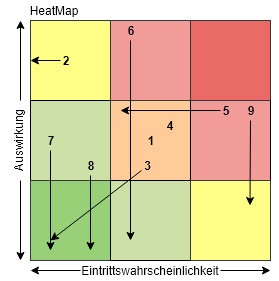
\includegraphics[scale=1]{graphics/HeatMap.PNG}
\caption{Heat Map}
\end{figure}

